
\section{Projection}

\begin{figure}[H]
    \centering
    \input{figures/projection_3d_courbe.tex}
    \caption{A control volume $\primal{K}$ and its projection $\projvariete \primal{K}$ onto the surface $\variete{M}$}
\end{figure}

\subsection{Global coordinates}

\cite[Sec. 2.3]{dziuk_finite_2013} Assume in the following that $G \subset \R^{n+1}$ is bounded and open with exterior normal $\nu$ and assume that $\variete{M} = \partial G$ is a $\Cont^k$-hypersurface ($k \geqslant 2$). The \defini{oriented distance function} for $\variete{M}$ is defined by
\[
d(x) \defeq \begin{cases}
\phantom{-} \inf\limits_{y \in \variete{M}} \abs{x - y} & x \in \R^{n+1} \setminus \overline{G} \\
- \inf\limits_{y \in \variete{M}} \abs{x - y} & x \in G
\end{cases}.
\]

\begin{figure}[H]
    \centering
    \tikzset{
    ddfv/.style={
        scale=1.5,
        every path/.style={thick,line join=round, cap=round},
        ptsq/.style 2 args={
          rectangle,
          fill=##1,
          inner sep=2pt,
          label={[text=##1]##2}
        },
        ptsqbord/.style 2 args={
          rectangle,
          draw=##1,
          inner sep=2pt,
          label={[text=##1]##2}
        },
        ptcl/.style 2 args={
          circle,
          fill=##1,
          inner sep=1.5pt,
          label={[text=##1]##2}
        },
        ptclbord/.style 2 args={
          circle,
          draw=##1,
          inner sep=1.5pt,
          label={[text=##1]##2}
        },
        mailleprimale/.style={
            myblue,
            fill=mylightblue
        },
        mailledualeint/.style={
            myred,
            fill=mylightred
        },
        mailledualebord/.style={
            myred,
            fill=mylightred!50!white
        },
        maillediamantint/.style={
            mygreen,
            fill=mylightgreen
        },
        maillediamantbord/.style={
            mygreen,
            fill=mylightgreen!50!white
        }
    }
}

\begin{tikzpicture}[
  ddfv
]

\def\largeur{3}
\def\ta{2.4}

% Courbe centrale
\def\f(#1){0.35*sin(1.0*#1 r)-0.15*#1}
\def\fp(#1){0.35*cos(1.0*#1 r)-0.15}

\draw[
  line width=\largeur cm,
  line cap=butt,
  line join=round,
  draw=mylightblue
]
plot[domain=0:6,samples=20,smooth] ({\x},{\f(\x)});

\draw plot[domain=0:6,samples=20,smooth] ({\x},{\f(\x)});

% Point a(x)
\pgfmathsetmacro{\ya}{\f(\ta)}
\pgfmathsetmacro{\slopea}{\fp(\ta)}
\pgfmathsetmacro{\nxa}{-\slopea/sqrt(1+\slopea^2)}
\pgfmathsetmacro{\nya}{1/sqrt(1+\slopea^2)}
\pgfmathsetmacro{\txa}{1/sqrt(1+\slopea^2)}
\pgfmathsetmacro{\tya}{\slopea/sqrt(1+\slopea^2)}

\pgfmathsetmacro{\dist}{0.6}
\pgfmathsetmacro{\xx}{\ta+\dist*\nxa}
\pgfmathsetmacro{\yx}{\ya+\dist*\nya}

\coordinate (P) at (\ta,\ya);

\draw[->, semithick] (P) -- ({\ta+1.2*\nxa},{\ya+1.2*\nya}) node[right] {$\vect{n}(\projvariete(x))$};

\def\eps{0.1}
\draw[semithick]
  (P)
  --
  ($(P)!-\eps cm!({\ta+\txa},{\ya+\tya})$)
  --
  ($($(P)!-\eps cm!({\ta+\txa},{\ya+\tya})$)!\eps cm!90:(P)$)
  --
  ($(P)!\eps cm!90:({\ta+\txa},{\ya+\tya})$)
  --
  cycle;

\node[ptcl={black}{below:$\projvariete(x)$}] at (P) {};
\node[ptcl={black}{left:$x$}] at (\xx,\yx) {};

\draw[myred, thick, <->] (P) -- (\xx,\yx) node[midway, right] {$d(x)$};

\pgfmathsetmacro{\yO}{\f(0)}
\pgfmathsetmacro{\slopeO}{\fp(0)}
\pgfmathsetmacro{\nxO}{-\slopeO/sqrt(1+\slopeO^2)}
\pgfmathsetmacro{\nyO}{1/sqrt(1+\slopeO^2)}

\pgfmathsetmacro{\distd}{\largeur/3}

\pgfmathsetmacro{\xd}{\distd*\nxO}
\pgfmathsetmacro{\yd}{\yO+\distd*\nyO}
\pgfmathsetmacro{\xdb}{-\distd*\nxO}
\pgfmathsetmacro{\ydb}{\yO-\distd*\nyO}

\draw[<->, semithick] (0,\yO) -- (\xd,\yd) node[midway, left] {$\delta$};
\draw[<->, semithick] (0,\yO) -- (\xdb,\ydb) node[midway, left] {$\delta$};

\node[myblue, above=10pt] at (1,{\f(1)}) {$U_\delta$};
\node[below] at (5.5,{\f(5.5)}) {$\surflisse$};

\end{tikzpicture}
    \caption{Strip $U_\delta$ around the hypersurface $\variete{M}$ and normal coordinates $x = \projvariete(x) + d(x) \, \nu(\projvariete(x))$}
\end{figure}

\begin{lemme}[{\cite[Lemma 2.8]{dziuk_finite_2013}}] \label{lemme:fermi_coordinates}
We define
\[
U_\delta \defeq \ens[\big]{x \in \R^{n+1} \tq \abs{d(x)} < \delta}.
\]
Then $d \in \Cont^k(U_\delta)$, and for every point $x \in U_\delta$ there exists a unique point $\projvariete(x) \in \variete{M}$ such that
\begin{equation} \label{eq:fermi_coordinates}
x = \projvariete(x) + d(x) \, \nu(\projvariete(x)).
\end{equation}
Moreover, we have that
\[
\grad d(x) = \nu(\projvariete(x)), \quad \abs{\grad d(x)} = 1, \quad \forall x \in U_\delta. 
\]
We also extend the normal constantly in the normal direction: $\nu(x) = \nu(\projvariete(x))$ for $x \in U_\delta$. Thus we have introduced a global coordinate system around $\variete{M}$. Every point $x \in U_\delta$ can be described by its \defini{Fermi coordinates} (normal coordinates) $d(x)$ and $\projvariete(x)$ according to \ref{eq:fermi_coordinates}.
\end{lemme}

\begin{envide}[\areprendre{À mettre dans régularité du maillage}]
\cite[Sec. 4.1]{dziuk_finite_2013} We assume that the surface $\variete{M}_h$ which approximates the smooth $n$-dimensional surface $\variete{M}$ ($\partial \variete{M} = \varnothing$) lies in the strip $U_\delta$ (see Lemma \ref{lemme:fermi_coordinates}) and is a Lipschitz surface. The strip can be chosen with locally varying width: see \ref{eq:eq41}. We assume that the discrete triangulated surface $\variete{M}_h$ besided \ref{eq:eq41} has the following properties. The surface $\variete{M}_h$ is the union of finitely many non-degenerate (closed) $n$-simplices in $\R^{n+1}$. We let $\ensprimal$ denote the set of these simplices:
\[
\variete{M}_h = \bigcup_{\primal{K} \in \ensprimal} \primal{K}. 
\]
The vertices $\enssomdual$ of the simplices are taken to sit on the smooth surface $\variete{M}$. For $\primal{K}, \primal{L} \in \ensprimal$, either $\primal{K} \cap \primal{L} = \varnothing$ or $\primal{K} \cap \primal{L}$ is an $(n-k)$-dimensional side simplex ($k \in \{1, \dots, n\}$) common to both of the simplices $\primal{K}$ and $\primal{L}$. For $\primal{K} \in \ensprimal$ we denote by $\diam{\primal{K}}$ its diameter and by $r(\primal{K})$ the in-ball radius. Also,
\[
h \defeq \max_{\primal{K} \in \ensprimal} \diam{\primal{K}}, \quad r \defeq \min_{\primal{K} \in \ensprimal} r(\primal{K}).
\]
We assume that the quantity
\[
\sigma \defeq \max_{\primal{K} \in \ensprimal} \sigma(\primal{K}), \quad \sigma(\primal{K}) = \frac{h(\primal{K})}{r(\primal{K})}
\]
is uniformly bounded independently of $h$.
\end{envide}

Note that, by Lemma \ref{lemme:fermi_coordinates}, for every simplex $\primal{K} \subset \variete{M}_h$ there is a unique curved simplex $\widetilde{\primal{K}} = \projvariete \primal{K} \subset \variete{M}$. In order to avoid global double covering, we assume that for each point $\projvariete \in \variete{M}$ there is at most one point $x \in \variete{M}_h$ with $\projvariete = \projvariete(x)$. This implies that there is a bijective correspondence between the triangles on $\variete{M}_h$ and the induced curvilinear triangles on $\variete{M}$.

We assume that $\variete{M}$ has only one connected component. We start with a discrete surface $\variete{M}_h$ contained in the variable strip $U_\delta$,
\begin{equation} \label{eq:eq41}
    \variete{M}_h \subset U_\delta = \ens[\big]{y + s \, \nu(y) \tq \abs{s} < \delta(y),\ y \in \variete{M}},
\end{equation}
where for a point $y \in \variete{M}$ we set
\[
\delta(y) = \min \bigg\{ \Big( \max_{i = 1, \dots, n} \abs{\kappa_i(y)} \Big)^{-1}, \sup_{z \in \variete{M}, z \not= y} \frac{L(y, z)}{\abs{y - z}} \bigg\}
\]
with the sectional curvatures $\kappa_i$ and where $L(y, z)$ denotes the geodesic distance between $y$ and $z$ on $\variete{M}$ (see \cite{lee_riemannian_1997} for the definitions of \defini{sectional curvature} and \defini{geodesic distance}). 

\begin{remarque}
    We can take $\delta \defeq \min_{y \in \variete{M}} \delta(y)$ which exists since $\variete{M}$ is a compact manifold. 
\end{remarque}

\begin{prop}
One can show that each point $x \in U_\delta$ can be uniquely projected onto the smooth surface, yielding the decomposition
\[
x = \projvariete(x) + d(x) \, \nu(\projvariete(x)), \quad x \in U_\delta,
\]
with $\projvariete(x)$ the orthogonal projection of $x$ onto $\variete{M}$ and $d(x)$ the oriented distance between $x$ and $\variete{M}$. 
\end{prop}

\begin{figure}[H]
    \centering
    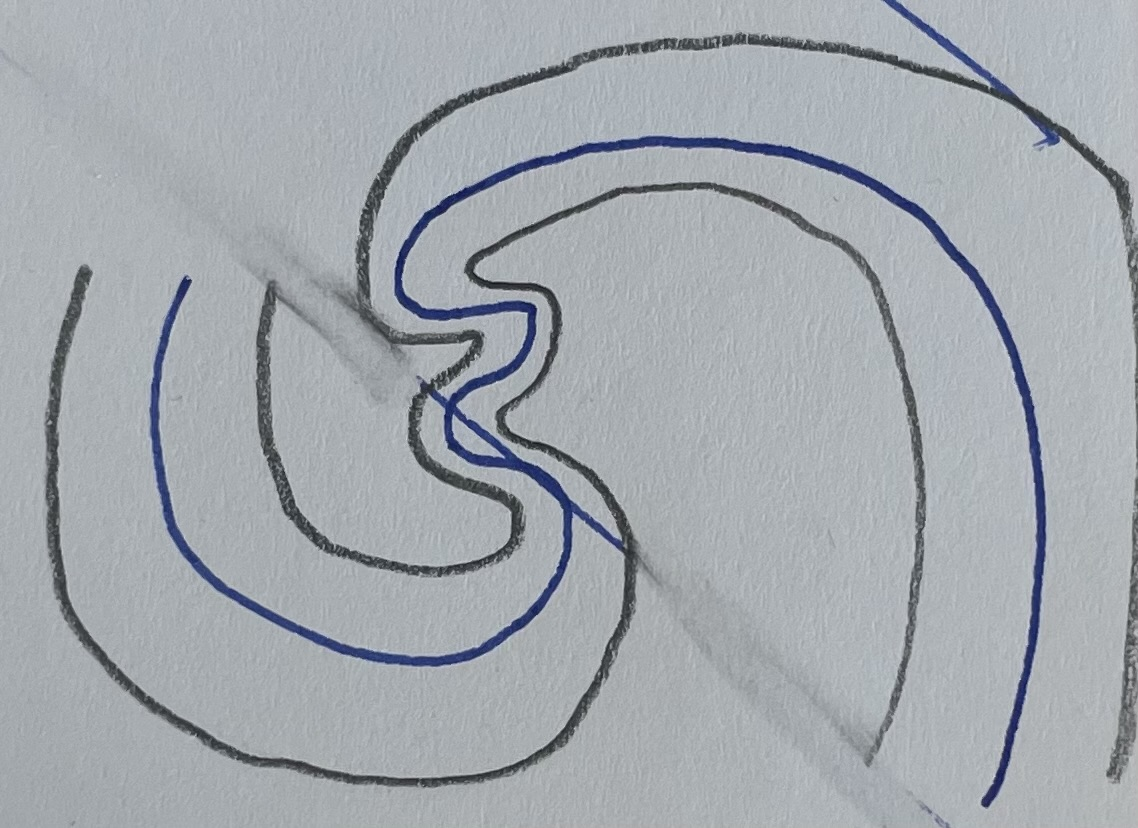
\includegraphics[width=0.5\textwidth]{img/strip_varying.jpeg}
    \caption{$\delta(y)$}
\end{figure}

\begin{prop}
\[
\variete{M} = \bigcup_{\primal{K} \in \ensprimal} \projvariete \primal{K}
= \bigcup_{\dual{K} \in \ensdual} \projvariete \dual{K}
= \bigcup_{\diamant{D} \in \ensdiamant} \projvariete \diamant{D}
\]
\end{prop}

\subsection{Approximation of geometry {\cite[Sec. 4.2]{dziuk_finite_2013}}}

We consider a piecewise linear approximation of a smooth surface $\variete{M} \in \Cont^2$ and its geometry. We collect estimates for the geometric error which is produced by approximating the smooth surface $\variete{M}$ by a discrete surface $\variete{M}_h$. 

\begin{figure}[H]
    \centering
    \tikzset{
    ddfv/.style={
        scale=1.5,
        every path/.style={thick,line join=round, cap=round},
        ptsq/.style 2 args={
          rectangle,
          fill=##1,
          inner sep=2pt,
          label={[text=##1]##2}
        },
        ptsqbord/.style 2 args={
          rectangle,
          draw=##1,
          inner sep=2pt,
          label={[text=##1]##2}
        },
        ptcl/.style 2 args={
          circle,
          fill=##1,
          inner sep=1.5pt,
          label={[text=##1]##2}
        },
        ptclbord/.style 2 args={
          circle,
          draw=##1,
          inner sep=1.5pt,
          label={[text=##1]##2}
        },
        mailleprimale/.style={
            myblue,
            fill=mylightblue
        },
        mailledualeint/.style={
            myred,
            fill=mylightred
        },
        mailledualebord/.style={
            myred,
            fill=mylightred!50!white
        },
        maillediamantint/.style={
            mygreen,
            fill=mylightgreen
        },
        maillediamantbord/.style={
            mygreen,
            fill=mylightgreen!50!white
        }
    }
}

\begin{tikzpicture}[
  ddfv,
  scale=6
]

\def\largeur{3}
\def\xL{1}

\def\f(#1){0.2*sin(pi*#1 r)}
\def\fp(#1){0.2*pi*cos(pi*#1 r)}

% \def\f(#1){0.2*sin(pi*#1^3 r)}
% \def\fp(#1){0.2*3*pi*#1^2*cos(pi*#1^3 r)}

\draw[myblue] (0.5,0.2) -- (0.5,{\f(\xL)+0.2}) node[midway, above] {$\projvariete \primal{K}$};
\draw[myblue] (0,0) -- (\xL,{\f(\xL)}) node[midway, below] {$\primal{K}$};

\draw plot[domain=-0.1:{\xL+0.1},samples=20,smooth] ({\x},{\f(\x)}) node[above right] {$\variete{M}$};

\node[ptsq={myblue}{}] at (0,0) {};
\node[ptsq={myblue}{}] at (\xL,{\f(\xL)}) {};

\foreach \ta in {0.1,0.2,...,0.9}
{
\pgfmathsetmacro{\ya}{\f(\ta)}
\pgfmathsetmacro{\slopea}{\fp(\ta)}
\pgfmathsetmacro{\txa}{1/sqrt(1+\slopea^2)}
\pgfmathsetmacro{\tya}{\slopea/sqrt(1+\slopea^2)}
\pgfmathsetmacro{\nxa}{-\slopea/sqrt(1+\slopea^2)}
\pgfmathsetmacro{\nya}{1/sqrt(1+\slopea^2)}
\pgfmathsetmacro{\xx}{\ta-\ya*\nxa/\nya}

\coordinate (P) at (\ta,\ya);

\draw[semithick] (P) -- (\xx, 0);

\def\eps{0.01}

\draw[semithick]
  (P)
  --
  ($(P)!\eps cm!({\ta+\txa},{\ya+\tya})$)
  --
  ($($(P)!\eps cm!({\ta+\txa},{\ya+\tya})$)!\eps cm!90:(P)$)
  --
  ($(P)!\eps cm!-90:({\ta+\txa},{\ya+\tya})$)
  --
  cycle;
}


\def\ta{0.3}

\pgfmathsetmacro{\ya}{\f(\ta)}
\pgfmathsetmacro{\slopea}{\fp(\ta)}
\pgfmathsetmacro{\txa}{1/sqrt(1+\slopea^2)}
\pgfmathsetmacro{\tya}{\slopea/sqrt(1+\slopea^2)}
\pgfmathsetmacro{\nxa}{-\slopea/sqrt(1+\slopea^2)}
\pgfmathsetmacro{\nya}{1/sqrt(1+\slopea^2)}
\pgfmathsetmacro{\xx}{\ta-\ya*\nxa/\nya}

\coordinate (P) at (\ta,\ya);

\draw[myblue] plot[domain=0:\xL,samples=20,smooth] ({\x},{\f(\x)});

\draw[myred] (P) -- (\xx, 0);
\node[ptcl={myred}{above:{$\projvariete(x)$}}] at (P) {};
\node[ptcl={myred}{below:{$x$}}] at (\xx, 0) {};


\end{tikzpicture}
    \caption{A curved simplex $\projvariete \primal{K}$ is parametrized over a planar one. Orthogonal projection onto the smooth surface $\variete{M}$}
\end{figure}

\begin{lemme}[Projection {\cite[Lemma 4.1]{dziuk_finite_2013}}] \label{lemme:projection_dziuk}
Assume $\variete{M}$ and $\variete{M}_h$ are as above. The map $\fonctionens[\projvariete]{\variete{M}_h}{\variete{M}}$ is bijective. For the oriented distance function to $\variete{M}$ we have the estimate
\[
\norme{d}_{\L^\infty(\variete{M}_h)} \leqslant c \, h^2.
\]
The quotient, $\delta_h$, between the smooth and discrete surface measures $\d A$ and $\d A_h$, defined by $\delta_h \d A_h = \d A$, satisfies
\[
\norme{1 - \delta_h}_{\L^\infty(\variete{M}_h)} \leqslant c \, h^2.
\]
Let $P$ and $P_h$ be the projections onto the tangent planes, $P_{ij} = \delta_{ij} - \nu_i \, \nu_j$, $P_{h,ij} = \delta_{ij} - \nu_{h,i} \, \nu_{h,j}$, and let
\[
R_h \defeq \frac{1}{\delta_h} P(I - d\mathcal{H}) P_h (I - d\mathcal{H}),
\]
$\mathcal{H}_{ij} = d_{x_i x_j} = \nu_{i_{x_j}}$. Then
\[
\norme{(I - R_h) P}_{\L^\infty(\variete{M}_h)} \leqslant c \, h^2.
\]
\end{lemme}

\begin{lemme}
{\color{red}
\[
\norme{d}_{\ensprimal + \ensdual} \leqslant c \, \size(\ensddfv)^2.
\]
}
\end{lemme}

\begin{lemme}
    \areprendre{À plat, $\mesure(\text{arête}) \sim h$ et $\mesure(\text{triangle}) \sim h^2$. Sur la surface aussi.}
\end{lemme}

\areprendre{
For any function $\eta$ defined on the discrete surface $\variete{M}_h$ we define an extension or lift onto $\variete{M}$ by
\begin{equation} \label{eq:lift}
\eta^\ell(a) = \eta(x(a)), \quad a \in \variete{M},    
\end{equation}
where, by our assumptions, $x(a)$ is defined as the unique solution of
\[
x = a + d(x) \, \nu(a).
\]
Furthermore, we understand by $\eta^\ell(x)$ the constant extension from $\variete{M}$ in the normal direction $\nu(a(x))$.

In order to compare the norms between functions on $\variete{M}_h$ and their lift \ref{eq:lift} to $\variete{M}$ we need the following lemma. 

\begin{lemme}
Let $\fonctionens[\eta]{\variete{M}_h}{\R}$ with the lift $\fonctionens[\eta^\ell]{\variete{M}}{\R}$. Then, for the plane $T \subset \variete{M}_h$, and smooth curved triangles $\widetilde{T} \subset \variete{M}$, the following estimates hold is the norm exist. There is a constant $c > 0$ independant of $h$ such that
\begin{align*}
    \frac{1}{c} \norme{\eta}_{\L^2(T)} &\leqslant \norme{\eta^\ell}_{\L^2(\widetilde{T})} \leqslant c \norme{\eta}_{\L^2(T)}, \\
    \frac{1}{c} \norme{\grad_{\variete{M}_h} \eta}_{\L^2(T)} &\leqslant \norme{\grad_{\variete{M}} \eta^\ell}_{\L^2(\widetilde{T})} \leqslant c \norme{\grad_{\variete{M}_h} \eta}_{\L^2(T)}, \\
    \norme{\grad^2_{\variete{M}_h} \eta}_{\L^2(T)} &\leqslant c \norme{\grad^2_{\variete{M}} \eta^\ell}_{\L^2(\widetilde{T})} + c \, h \norme{\grad_{\variete{M}} \eta^\ell}_{\L^2(\widetilde{T})}.
\end{align*}
\end{lemme}
}

\subsection{Discrete charts {\cite[Sec. 4.3]{dziuk_finite_2013}}}

\areprendre{
We add some information on a discrete differential geometric approach which is consistent with the introduction of parametrized surfaces. For a complete exposition see Nedelec (1976). 

Let $\variete{M}$ be given as in Section 2.1 by local charts $(X_i)_{i \in I}$, $X_i \in \Cont^k(V_i, \R^{n+1})$. We assume that already
\[
\variete{M} = \bigcup_{i \in I} X_i(V_{ih}),
\]
with $V_{ih} \subset V_i$ and triangulated domains $V_{ih} \subset \R^n$. We interpolate the smooth parametrization $X_{ih} = I_h X_i$, where $I_h$ is the interpolation from Lemma 4.3 on the polygonal domain $V_{ih}$. We assume that if $U_{ij} = X_{ih}(V_{ih}) \cap X_{jh}(V_{jh}) \not= \varnothing$, then the map $\fonctionens[X_{ih}{}^{-1} \circ X_{jh}]{X_{jh}{}^{-1}(U_{ij})}{X_{ih}{}^{-1}(U_{ij})}$ is bijective, continuous and piecewise linear. The the discrete surface is defined by
\[
\variete{M}_h = \bigcup_{i \in I} X_{ih}(V_{ih}).
\]
The advantage of this way to discretize the surface $\variete{M}$ is that it allows the approximation of immersions. 
}